\documentclass[12pt]{article}
\usepackage[margin=1in]{geometry}
\usepackage{amsmath,amssymb}
\usepackage{graphicx}
\usepackage{booktabs,array}
\usepackage{longtable}
\usepackage{caption}

\renewcommand{\thetable}{S\arabic{table}}
\renewcommand{\thefigure}{S\arabic{figure}}

\begin{document}

\begin{center}
{\Large Electronic supplementary material}\\[0.5em]
{\large Benchmark-conditioned transformation uncertainty in aquifer-test parameter interpretation}\\[0.5em]
Ying-Fan Lin\\
Department of Civil Engineering, Chung Yuan Christian University, Taoyuan, Taiwan\\
\texttt{yflin1110@cycu.edu.tw}
\end{center}

\section*{Supplementary tables}

\begin{table}[!htbp]
\centering
\footnotesize
\setlength{\tabcolsep}{4pt}
\renewcommand{\arraystretch}{0.95}
\caption{Uncertainty source matrix for separation of field response diagnostics, parameter compensation, and unresolved uncertainty sources.}
\label{tab:s_uncertaintysources}
\begin{tabular}{@{}p{0.25\linewidth}p{0.67\linewidth}@{}}
\toprule
Source & Evidence and current limitation \\
\midrule
Inherent variability & Field COV and variance after removing the trend diagnose variability in inferred hydraulic properties; independent heterogeneity remains a separate evidence need. \\
Measurement error & The Lovelock detection threshold is included; the Massachusetts site instrument budget remains unavailable. \\
Pumping schedule and preprocessing & Massachusetts retained constant rate analysis and Lovelock pumping/recovery superposition are reported separately. \\
Transformation uncertainty & Time and well indexed log model factor dispersion, model factor distributions, diagnostics by time window, and consistency between the two field cases quantify interpretation related response uncertainty. \\
Model form & AIC/BIC, model definitions, leakage support, and boundary diagnostics compare implemented interpretation models and expose unimplemented model limits. \\
Statistical and identifiability & Local MAP correlations, boundary flags, leakage support, and field parameter COV diagnose finite sample and tradeoff effects. \\
Support and decision scale & Spatial transfer, comparison between the two field cases, Bayesian model averaging, robust hydraulic control capacity factors, and response time consequences connect parameter estimation to groundwater use. \\
\bottomrule
\end{tabular}
\end{table}

\begin{table}[!htbp]
\centering
\scriptsize
\setlength{\tabcolsep}{2.2pt}
\renewcommand{\arraystretch}{0.95}
\caption{Parallel headline results for the Massachusetts and Lovelock Valley field cases across the model sequence Theis confined / Hantush--Jacob leaky / lagging Darcy without leakage / lagging Darcy with leakage.}
\label{tab:s_headline}
\begin{tabular}{@{}p{0.25\linewidth}p{0.34\linewidth}p{0.34\linewidth}@{}}
\toprule
Evidence item & Massachusetts field case & Lovelock Valley field case \\
\midrule
Setting and support & Fractured bedrock; 5.8--36.6 m radial support & Basin fill aquifer; 0.6--9.6 mi radial support \\
Wells / response records & 12 / 420 & 7 / 520 \\
Observation design & Retained constant rate drawdown subset & Pumping and recovery superposition with 0.05 ft detection offset \\
Pooled log model factor $SD_{\epsilon}$ & 0.166 / 0.164 / 0.062 / 0.035 & 0.246 / 0.294 / 0.174 / 0.174 \\
BIC preferred wells & 2 / 2 / 3 / 5 & 2 / 0 / 5 / 0 \\
Transmissivity COV & 0.58 / 0.78 / 0.46 / 0.81 & 3.40 / 3.70 / 1.83 / 4.77 \\
Storage COV & 2.05 / 1.71 / 1.74 / 1.54 & 0.89 / 0.86 / 0.95 / 10.21 \\
Support for models that include leakage & Lagging leaky BIC preferred in 5 wells, with spatially selective leakage support & BIC preference concentrated in models without leakage \\
Scope of validation & Spatial transfer diagnostic available for the small well network & Field consistency check available for the processed regional data set \\
\bottomrule
\end{tabular}
\end{table}

\begin{table}[!htbp]
\centering
\scriptsize
\setlength{\tabcolsep}{2.0pt}
\renewcommand{\arraystretch}{0.95}
\caption{Model-averaged management diagnostic for aquifer-test transformation uncertainty across the four formally fitted analytical interpretations, Theis confined, Hantush--Jacob leaky, lagging Darcy without leakage, and lagging Darcy with leakage. Rows without a strict BIC prefix use variance-window BMA weights.}
\label{tab:s_decisionconsequence}
\begin{tabular}{@{}p{0.38\linewidth}p{0.28\linewidth}p{0.28\linewidth}@{}}
\toprule
Decision diagnostic & Massachusetts field case & Lovelock Valley field case \\
\midrule
Mean model weights & 0.19 / 0.22 / 0.26 / 0.32 & 0.25 / 0.15 / 0.34 / 0.26 \\
Selected model counts & 2 / 2 / 3 / 5 & 2 / 0 / 5 / 0 \\
Strict BIC median capacity factor & 1.00 & 1.00 \\
Median capacity factor & 1.60 & 1.18 \\
95th percentile capacity factor & 2.73 & 4.52 \\
Mean capacity shortfall probability & 0.38 & 0.21 \\
Median response factor & 1.85 & 4.05 \\
95th percentile response factor & 3.32 & 8.79 \\
Mean earlier response probability & 0.41 & 0.23 \\
Median diffusivity spread & 1.90 & 3.91 \\
\bottomrule
\end{tabular}
\end{table}

\begin{table}[!htbp]
\centering
\footnotesize
\setlength{\tabcolsep}{3.0pt}
\renewcommand{\arraystretch}{0.95}
\caption{Groundwater report endpoint for aquifer-test transformation uncertainty via the evidence sequence from measured response to numerical benchmark support, field applicability, and decision consequence.}
\label{tab:s_reportingframework}
\begin{tabular}{@{}>{\raggedright\arraybackslash}p{0.24\linewidth}>{\raggedright\arraybackslash}p{0.70\linewidth}@{}}
\toprule
Reporting item & Required statement before pumping-test-derived hydraulic properties are used \\
\midrule
Measured response and support & State the pumping representation, observation geometry, detection threshold or offset, and retained well records so that the transformed response and spatial support are explicit. \\
Interpretation model & Identify whether $T$ and $S$ come from Theis confined, Hantush--Jacob leaky, lagging Darcy without leakage, lagging Darcy with leakage, or another stated interpretation. \\
Response log model factor & Report observed-predicted log response diagnostics and pooled $SD_{\epsilon}$ for each interpretation to make response-level transformation error visible. \\
Complexity and parameter spread & Report information criteria, leakage or boundary support, fitted parameter COV, and identifiability flags before interpreting apparent parameters as hydrogeologic evidence. \\
Numerical model factor support & Use screened benchmark model factor distributions for matching scenario classes, pathways, and observation supports. \\
Field applicability check & State the field-to-benchmark class match after response, residual, complexity, and parameter-spread diagnostics so the scenario-conditioned COV values are tied to their support. \\
Decision consequence & Propagate the supported interpretation set to capacity, diffusivity, and response-time diagnostics so later groundwater control or management calculations know what uncertainty they inherit. \\
\bottomrule
\end{tabular}
\end{table}

\clearpage
\section*{Supplementary figures}

\begin{figure}[!htbp]
\centering
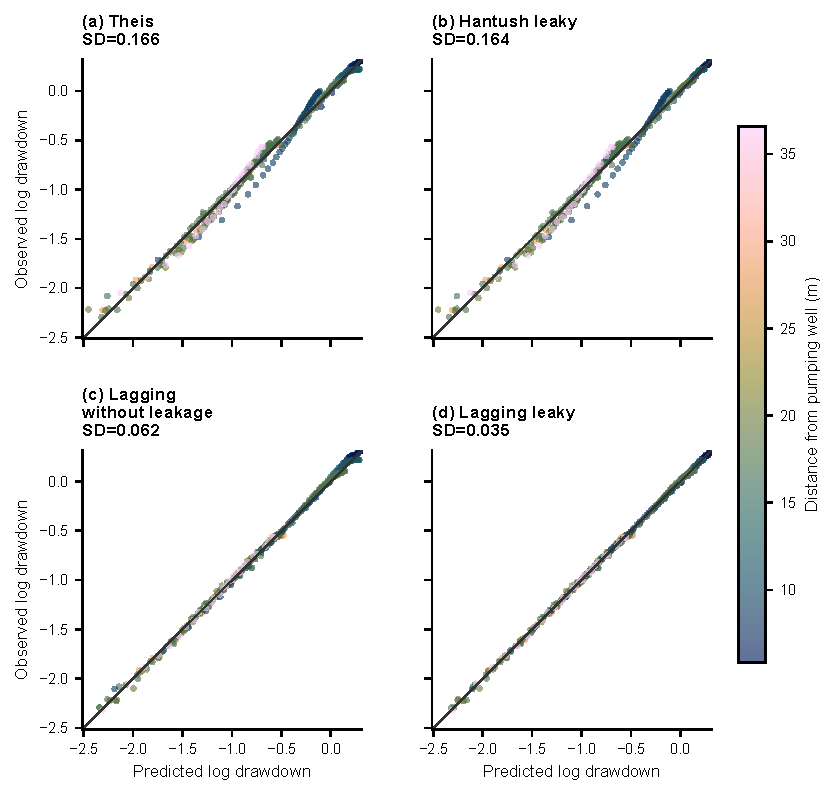
\includegraphics[width=\linewidth]{fig04_transformation_scatter.pdf}
\caption{Massachusetts observed and predicted log drawdown comparison across (a) Theis confined; (b) Hantush--Jacob leaky; (c) lagging Darcy without leakage; and (d) lagging Darcy with leakage, with marker color for distance from the extraction well.}
\label{fig:s_scatter}
\end{figure}

\begin{figure}[!htbp]
\centering
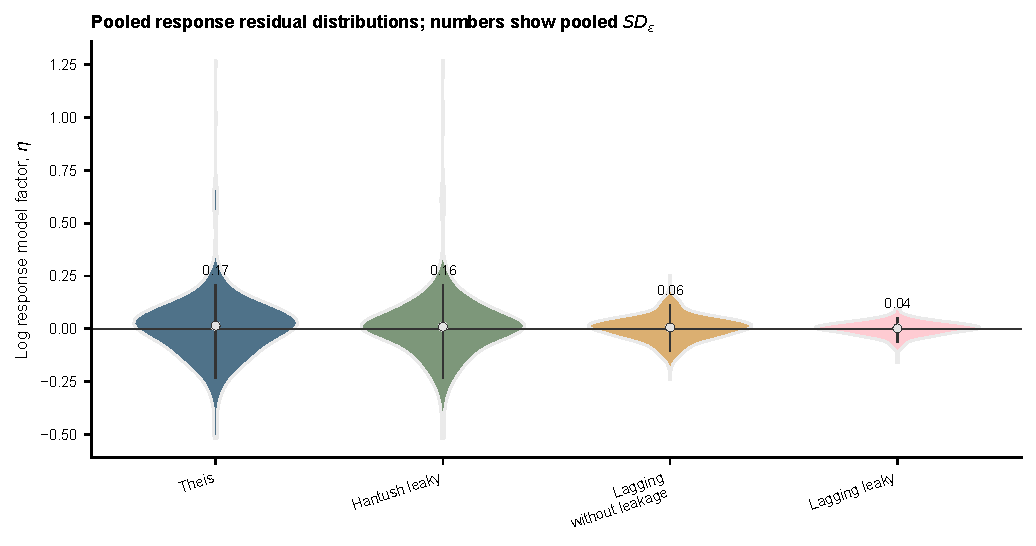
\includegraphics[width=0.92\linewidth]{fig05_transformation_residual_distributions.pdf}
\caption{Massachusetts log model factor distributions across (a) Theis confined; (b) Hantush--Jacob leaky; (c) lagging Darcy without leakage; and (d) lagging Darcy with leakage, with vertical intervals for the 5th--95th percentile range, markers for medians, and numeric labels for pooled $SD_{\epsilon}$.}
\label{fig:s_residualdist}
\end{figure}

\begin{figure}[!htbp]
\centering
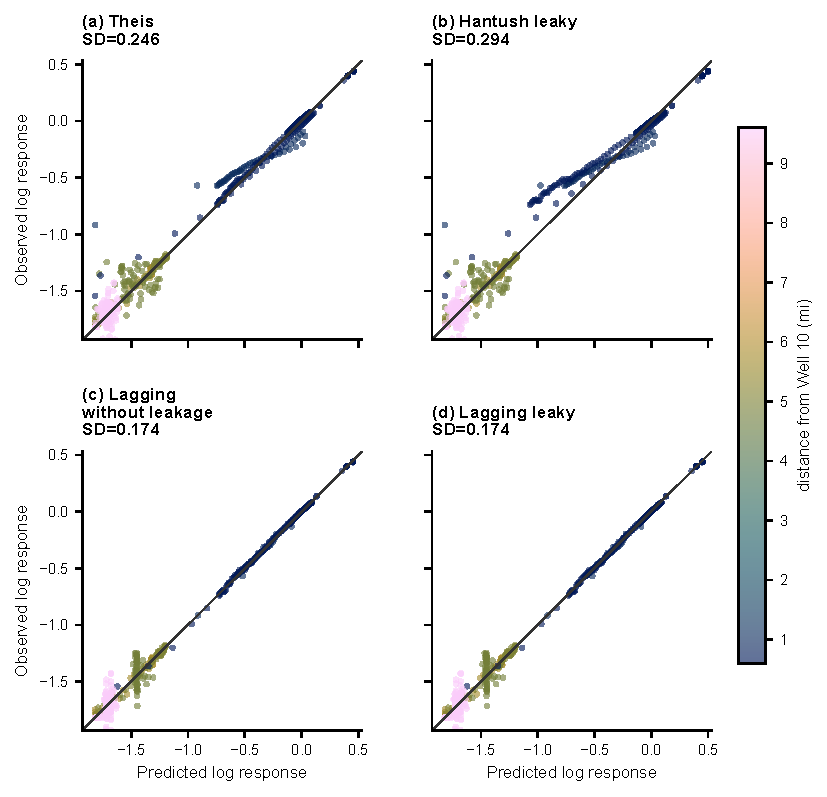
\includegraphics[width=\linewidth]{fig08_lovelock_transformation_scatter.pdf}
\caption{Lovelock Valley observed and predicted log response comparison across (a) Theis confined; (b) Hantush--Jacob leaky; (c) lagging Darcy without leakage; and (d) lagging Darcy with leakage, with marker color for distance from Well 10.}
\label{fig:s_lovelockscatter}
\end{figure}

\begin{figure}[!htbp]
\centering
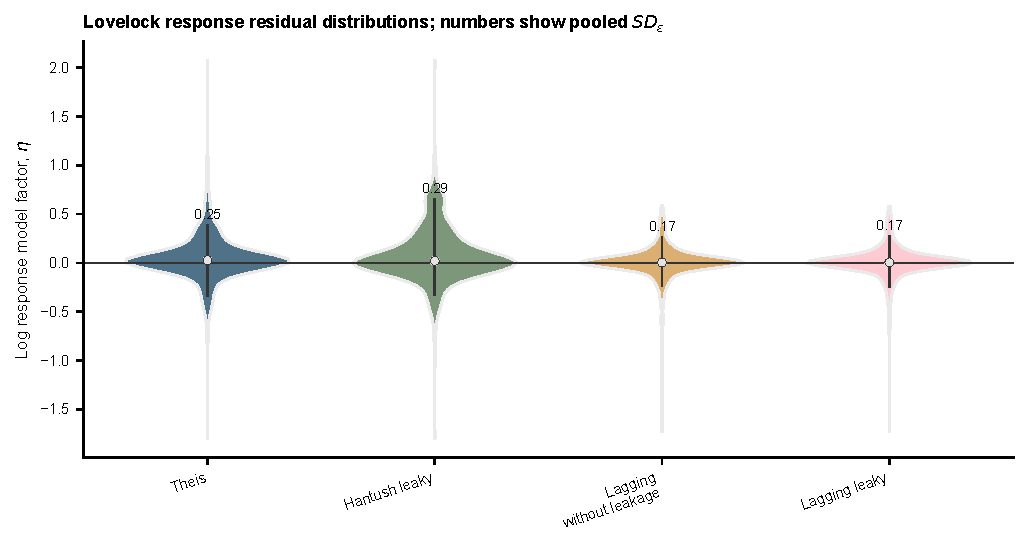
\includegraphics[width=0.92\linewidth]{fig09_lovelock_residual_distribution.pdf}
\caption{Lovelock Valley log model factor distributions across (a) Theis confined; (b) Hantush--Jacob leaky; (c) lagging Darcy without leakage; and (d) lagging Darcy with leakage, with vertical intervals for the 5th--95th percentile range, markers for medians, and numeric labels for pooled $SD_{\epsilon}$.}
\label{fig:s_lovelockresidual}
\end{figure}

\end{document}
